%TCIDATA{LaTeXparent=0,0,cap_RevisaoBibliografica.tex}

\section{Simula\c{c}\~{a}o Num\'{e}rica de Reservat\'{o}rios}
\subsection{Visão Geral}
A simula\c{c}\~{a}o num\'{e}rica de um reservat\'{o}rio \'{e}, segundo Peaceman, \'{e} o processo de infer\^{e}ncia do comportamento do reservat\'{o}rio real dada a performance obtida de um modelo do mesmo, matem\'{a}tico ou f\'{i}sico (em escala laboratorial). Um modelo matem\'{a}tico de reservat\'{o}rio pode ser enxergado como um conjunto de equa\c{c}\~{o}es diferenciais parciais, juntamente com as condi\c{c}\~{o}es de contorno adequadas, que podem ser utilizadas para descrever satisfatoriamente os processos f\'{i}sicos importantes que ocorrem no sistema real. Os processos que ocorrem em um reservat\'{o}rio s\~{a}o basicamente transporte de fluidos e transfer\^{e}ncia de massa; at\'{e} tr\^{e}s fases imisc\'{i}veis (\'{o}leo, g\'{a}s e \'{a}gua) fluem simultaneamente, enquanto que o transporte de massa se d\'{a} entre as fases (notadamente entre o \'{o}leo e o g\'{a}s). A gravidade, a capilaridade e as for\c{c}as viscosas s\~{a}o tamb\'{e}m importantes no processo de vaz\~{a}o dos fluidos \cite{simres}.

Além da definição proposta por Peaceman, Heimsund descreve a simulação de reservatórios como uma ferramenta de investigação da vazão de fluidos em subsuperfície. O autor destaca que as simulações de reservatório abrangem áreas relacionadas a ramos importantes da ciência, como matemática, física, química, geologia e biologia; além disso, afirma que, na indústria petrolífera, os principais usos dos simuladores de reservatórios envolvem a obtenção de esquemas ótimos de explotação e predição da produção\cite{heimsund2005}. Já Dake afirma que um simulador numérico de reservatório é um programa de computador em que o sistema estudado é dividido em várias células discretas, cujas propriedades podem ser diferentes entre si \cite{dake}.

Segundo Rosa, a primeira etapa de uma simula\c{c}\~{a}o num\'{e}rica \'{e} formular o problema f\'{i}sico a ser representado matematicamente; em seguida s\~{a}o feitas suposi\c{c}\~{o}es e simplifica\c{c}\~{o}es compat\'{i}veis com o grau de sofistica\c{c}\~{a}o esperado do modelo, levando-se \`{a} formula\c{c}\~{a}o das equa\c{c}\~{o}es matem\'{a}ticas que descrevem o problema desejado, considerando-se as hip\'{o}teses adotadas. O passo seguinte \'{e} a resolu\c{c}\~{a}o das equa\c{c}\~{o}es e an\'{a}lise da solu\c{c}\~{a}o obtida; posteriormente, a validade do simulador \'{e} verificada atrav\'{e}s da calibra\c{c}\~{a}o com uma solu\c{c}\~{a}o existente --- por exemplo, comparam-se os resultados obtidos do simulador num\'{e}rico com solu\c{c}\~{o}es anal\'{i}ticas, resultados reais ou com resultados obtidos de modelos f\'{i}sicos de laborat\'{o}rio (dados experimentais). Caso o simulador seja considerado v\'{a}lido, o mesmo estar\'{a} pronto para ser utilizado na simula\c{c}\~{a}o do fen\^{o}meno desejado; caso contr\'{a}rio, volta-se para um novo ciclo em que s\~{a}o revistas as hip\'{o}teses adotadas ou at\'{e} a conceitua\c{c}\~{a}o do modelo f\'{i}sico \cite[p. 520]{engres}. A Figura \ref{fig:rev_simuesq} esquematiza um desenvolvimento b\'{a}sico de um simulador num\'{e}rico qualquer, enquanto que a Figura \ref{fig:rev_simuex} mostra uma compara\c{c}\~{a}o de resultados entre diferentes simuladores existentes, exemplificando o uso da calibra\c{c}\~{a}o com solu\c{c}\~{o}es j\'{a} obtidas para se validar um simulador de reservat\'{o}rio. 

\begin{figure}[H]
\centering
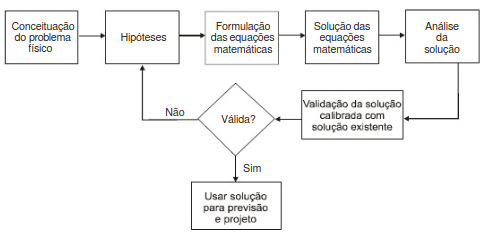
\includegraphics[width=.75\textwidth]{figs/revisao/revisao_simuesq.png}
\caption{Esquema b\'{a}sico de desenvolvimento de um simulador num\'{e}rico de reservat\'{o}rio \cite[p. 519]{engres}.}\label{fig:rev_simuesq}
\end{figure}

\begin{figure}[H]
\centering
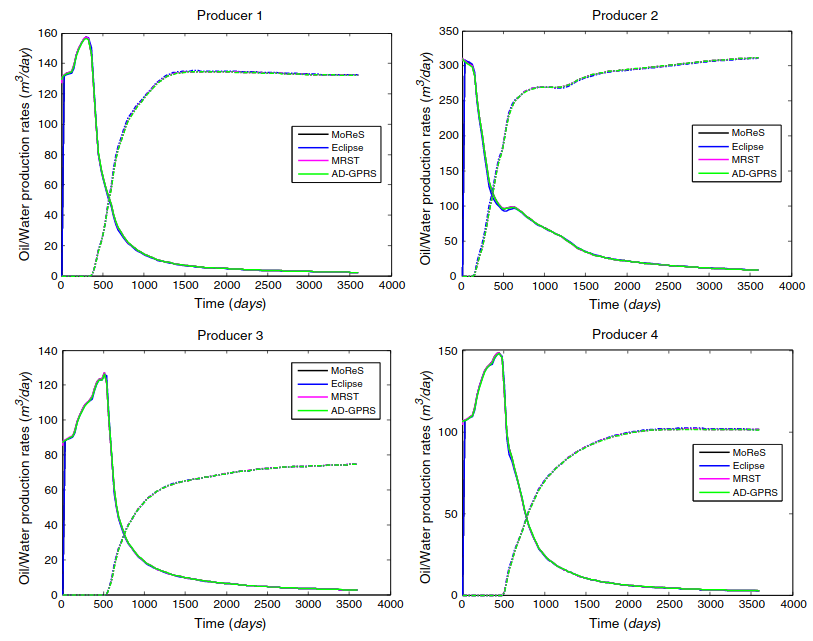
\includegraphics[width=.75\textwidth]{figs/revisao/revisao_simuex.png}
\caption{Exemplo de compara\c{c}\~{a}o de dados entre simuladores de vaz\~{a}o de \'{a}gua e de \'{o}leo de um modelo \cite{eggM}.}\label{fig:rev_simuex}
\end{figure}

\subsection{História da Simulação de Reservatórios}
Para se traçar a evolução da simulação de reservatórios ao longo da história, consideram-se aqui, inicialmente, fatos apresentados por Coats e por Breitenbach; de acordo com Coats, a simulação de reservatórios é praticada desde o surgimento da engenharia de petróleo, durante a década de 1930. Já na década de 1940, segundo Breitenbach, a simulação de reservatórios passa a ser reconhecida, com as companhias desenvolvendo métodos analíticos e numéricos para a melhoria das soluções analíticas resistentes, balanço de materiais e cálculo de posicionamento 1-D de Buckley-Leverett; na década seguinte (1950), as pesquisas por soluções numéricas das equações de vazão começam a surtir efeito, com o surgimento de programas computacionais rudimentares, porém eficientes, de simulações de reservatórios. Considera-se um grande avanço o surgimento dessas soluções, em que foi possível resolver equações de diferenças finitas em modelos 2D e 3D, além de simulações em meios de porosidade heterogênea; enfim, problemas mais complexos de engenharia de reservatório podiam ser resolvidos\footnote{Ver \cite{coats1982} e \cite{breitenbach1991}}.

A década de 1960 representou, segundo Coats, um marco importante, em que a palavra ``simulação'' se torna comum, à medida em que os programas destinados à resolução de problemas de reservatórios se tornavam mais sofisticados; durante essa década, os esforços na busca de simuladores melhores de reservatórios se concentraram em modelos bifásicos de gás/água e \textit{black-oil} trifásicos; os métodos de recuperação de óleo simulados se restringiam essencialmente à depleção ou manutenção da pressão. Era possível, na época, o desenvolvimento de um único modelo de simulação que conseguia tratar de quase todos os problemas de reservatórios encontrados, o que sempre atraiu o interesse das companhias operadoras do ramo por conta da redução de custos com treinamento e uso e, potencialmente, de custos de manutenção e desenvolvimento do modelo \cite{coats1982}.

Para se entender o rumo das simulações de reservatório na década de 1970, é importante considerar o momento histórico; nessa época, ocorria o embargo da OPEP (Organização dos Países Exportadores de Petróleo), acarretando um aumento brusco do preço do petróleo. Esse embargo, segundo Brosche, ocorreu como uma represália dos países árabes aos Estados Unidos e à União Europeia, devido ao apoio dos mesmos ao Estado de Israel durante as guerras que afetaram o Oriente Médio, uma região rica em petróleo; o embargo se deu logo após a guerra do Yom Kippur, em 1973 \cite{brosche1974}. Durante esse período, ocorre a proliferação dos métodos de EOR, como injeções miscíveis, químicas, de $CO_2$ e vapor, além da combustão \textit{in-situ}; os simuladores, portanto, passaram a considerar esses métodos de recuperação, além de adicionar aos modelos efeitos térmicos e comportamentos complexos de equilíbrio de fase. A estratégia de se manter um modelo único de reservatório, devido ao advento dos métodos de EOR, foi modificada com a ideia de se obter vários modelos reproduzindo o comportamento do sistema estudado em resposta aos métodos de recuperação de óleo aplicados. Pode-se afirmar, portanto, que a década de 1970 representou um avanço significativo no esforço de se obter simulações mais complexas, com custo computacional reduzido e melhor eficiência das soluções numéricas \cite{coats1982}.




\subsection{Leis F\'{i}sicas Consideradas}

No caso de um simulador de reservat\'{o}rios, as seguintes leis f\'{i}sicas b\'{a}sicas normalmente s\~{a}o consideradas, dependendo do tipo de simulador\footnote{Ver \cite[p. 520]{engres}}:

\begin{itemize}
\item Lei da conserva\c{c}\~{a}o de massa;
\item Lei da conserva\c{c}\~{a}o de energia;
\item Lei da conserva\c{c}\~{a}o de \textit{``momentum''} (Segunda Lei de Newton):
\begin{equation}
\sum F = \frac{\partial M}{\partial t},
\end{equation}
onde $F$ representa uma for\c{c}a e $M = mv$ o \textit{``momentum''}, com $m$ sendo a massa e $v$ a velocidade.
\end{itemize}

De um modo geral, na modelagem de fenômenos físicos, considera-se importante o estudo das equações de conservação; segundo Heimsund, o princípio da conservação pode ser generalizado tomando-se uma variável quantitativa $u$ contida em um volume de controle fixo $\Omega$. A variável $u$ pode ser modificada dentro de $\Omega$ por um dado fluxo $\vec{F}$ sobre a superfície de contorno $\Gamma$ de $\Omega$. A conservação de $u$ pode ser escrita, na sua forma integral, como
\begin{equation}
	\int_{\Omega} \frac{\partial u}{\partial t}dV ~+~\oint_{\Gamma}\vec{F}\cdot\vec{n}dS = \int_{\Omega} Q dV,
\end{equation}
em que $Q$ pode ser encarado como uma fonte ($Q > 0$) ou dreno ($Q < 0$). A integral de superfície pode ser convertida, utilizando-se o teorema de Gauss; portanto, a equação da conservação de $u$ pode ser reescrita como
\begin{equation}
\int_{\Omega} \frac{\partial u}{\partial t}dV + \int_{\Omega} \nabla\cdot\vec{F} dV = \int_{\Omega}Q dV
\end{equation}
\begin{equation}\label{consU}
\int_{\Omega} \left(\frac{\partial u}{\partial t} + \nabla\cdot\vec{F} - Q \right)dV = 0.
\end{equation}
Como a Equação \eqref{consU} deve valer para qualquer tamanho de $\Omega$, a integral pode ser omitida da equação:
\begin{equation}\label{consU2}
\frac{\partial u}{\partial t} + \nabla\cdot\vec{F} = Q.
\end{equation}
No caso da modelagem de fluxo em reservatório, a variável $u$ pode ser, por exemplo, a massa de uma dada fase (água, óleo ou gás), a massa molecular das substâncias ou a energia térmica \cite{heimsund2005}.

Al\'{e}m das leis b\'{a}sicas da f\'{i}sica, faz-se necess\'{a}rio o uso de v\'{a}rias leis, dependendo do simulador, que governam o comportamento dos fluidos envolvidos e a propriedade do reservat\'{o}rio estudado, apresentadas nas subse\c{c}\~{o}es a seguir\footnote{Os teoremas apresentados se encontram em \cite[pp. 520-522]{engres}}. Combinado-se as equa\c{c}\~{o}es correspondentes \`{a}s leis b\'{a}sicas, obt\'{e}m-se uma equa\c{c}\~{a}o diferencial parcial que rege o comportamento das vari\'{a}veis dependentes em fun\c{c}\~{a}o das vari\'{a}veis independentes e dos par\^{a}metros do sistema. Como normalmente a equa\c{c}\~{a}o obtida \'{e} n\~{a}o-linear, ela \'{e}, consequentemente, \'{e} resolvida por m\'{e}todos n\'{u}mericos; da\'{i} a nomenclatura \textit{simula\c{c}\~{a}o num\'{e}rica de reservat\'{o}rios}. 

\subsubsection{Fen\^{o}menos de Transporte}

\begin{theorem}[Lei de Darcy]
Na Lei de Darcy, ou lei do fluxo ``laminar'' ou Darcyano, a velocidade do fluxo viscoso de um fluido em meio poroso \'{e} dada por
\begin{equation}
	v_s = -\frac{k_s}{\mu} \frac{\partial\Phi}{\partial s},
\end{equation}
onde $k$ \'{e} a permeabilidade efetiva do meio ao fluido considerado, $\mu$ \'{e} a viscosidade do fluido, $\Phi$ \'{e} o potencial de fluxo e $s$ \'{e} a trajet\'{o}ria de fluxo.
\end{theorem}

\begin{theorem}[Lei de Forchheimer]
Tamb\'{e}m conhecida como lei do fluxo ``turbulento'' ou n\~{a}o-Darcyano, \'{e} utilizada para fluxos turbulentos, notadamente de g\'{a}s; o gradiente de press\~{a}o \'{e} dado por
\begin{equation}
	-\frac{dp}{ds} = \frac{\mu}{k_s}v_s - \beta\rho v_s^2,
\end{equation}
onde $\rho$ \'{e} a massa espec\'{i}fica do fluido e $\beta$ \'{e} o coeficiente de resist\^{e}ncia inercial ou de fluxo n\~{a}o-Darcyano. 
\end{theorem}

\begin{theorem}[Lei de Fourier]
Durante um fen\^{o}meno de transporte de calor por condu\c{c}\~{a}o, o fluxo de calor \'{e} dado por
\begin{equation}
	q_s = -k'\frac{\partial T}{\partial s},
\end{equation}
em que $k'$ \'{e} a condutividade t\'{e}rmica do meio e $T$ \'{e} a temperatura.
\end{theorem}

\begin{theorem}[Convec\c{c}\~{a}o]
O fluxo de calor no caso de tranporte por convec\c{c}\~{a}o \'{e} dado por
\begin{equation}
	q_s = c_p v_s (T - T_0),
\end{equation}
onde $c_p$ \'{e} a capacidade calor\'{i}fica do fluido \`{a} press\~{a}o constante, $v$ a velocidade do fluido e $T_0$ uma temperatura de refer\^{e}ncia.
\end{theorem}

\subsubsection{Equa\c{c}\~{o}es de Estado}
As principais equa\c{c}\~{o}es de estado envolvidas na simula\c{c}\~{a}o do comportamento de um reservat\'{o}rio de petr\'{o}leo s\~{a}o as que lidam com fluidos (l\'{i}quidos ou gasosos) e rochas porosas. No caso de fluidos l\'{i}quidos, tem-se a seguinte defini\c{c}\~{a}o:

\begin{definition}
A compressibilidade isot\'{e}rmica de um fluido \'{e} dada por
\begin{equation}
	c = -\frac{1}{V}\frac{\partial V}{\partial p} = \frac{1}{\rho}\frac{\partial \rho}{\partial p},
\end{equation}
em que $V$ \'{e} o volume, $p$ \'{e} a press\~{a}o e $\rho$ \'{e} a massa espec\'{i}fica do fluido. H\'{a} algumas rela\c{c}\~{o}es especiais para situa\c{c}\~{o}es particulares:
\begin{itemize}
\item L\'{i}quidos de compressibilidade constante: $\rho = \rho_0 e^{c(p-p_0)}$.
\item L\'{i}quidos de compressibilidade constante e pequena: $\rho = \rho_0 \left[1+c\left(p-p_0\right)\right]$.
\end{itemize}
\end{definition}

Quando se trata de estudar o estado de um g\'{a}s, se aplica a lei dos gases:
\begin{equation}\label{eq:gaslaw}
	\rho = \frac{pM}{ZRT}.
\end{equation}

A Equa\c{c}\~{a}o \eqref{eq:gaslaw} pode ser aplicada tanto no caso de um g\'{a}s real quanto de um g\'{a}s ideal; nela, $\rho$ \'{e} a massa espec\'{i}fica do g\'{a}s, $p$ \'{e} a press\~{a}o, $M$ \'{e} a massa molecular, $R$ \'{e} a constante universal dos gases, $T$ \'{e} a temperatura e $Z$ \'{e} o fator de compressibilidade do g\'{a}s; no caso de um g\'{a}s ideal, tem-se $Z = 1$.

Por fim, para se representar o comportamento da rocha, utiliza-se a equa\c{c}\~{a}o da chamada compressibilidade efetiva:
\begin{equation}
	c_f = \frac{1}{\phi} \frac{\partial\phi}{\partial p},
\end{equation}
onde $c_f$ \'{e} a compressibilidade efetiva efetiva da forma\c{c}\~{a}o e $\phi$, sua porosidade.

Al\'{e}m das leis at\'{e} aqui citadas, cabe ressaltar que outras podem ser utilizadas em caso de simula\c{c}\~{o}es de fen\^{o}menos espec\'{i}ficos, como inje\c{c}\~{a}o de vapor, inje\c{c}\~{a}o de pol\'{i}meros, al\'{e}m de outros m\'{e}todos empregados na produ\c{c}\~{a}o de petr\'{o}leo.

\subsection{Tipos de Simuladores}
Segundo Rosa, os simuladores de reservat\'{o}rios podem ser classificados em fun\c{c}\~{a}o de tr\^{e}s crit\'{e}rios b\'{a}sicos: o tratamento matem\'{a}tico utilizado, o n\'{u}mero de dimens\~{o}es consideradas e o n\'{u}mero de fases admitidas. Em rela\c{c}\~{a}o \`{a} matem\'{a}tica do simulador, os simuladores podem ser classificados em: 

\begin{itemize}
	\item \textbf{Modelo Beta ou volum\'{e}trico:} \'{e} tamb\'{e}m conhecido como \textit{black oil}; nesse modelo, s\~{a}o consideradas as fun\c{c}\~{o}es de press\~{a}o e da temperatura do reservat\'{o}rio. Al\'{e}m disso, cada fase presente no reservat\'{o}rio (\'{a}gua, \'{o}leo e/ou g\'{a}s) \'{e} admitida como constitu\'{i}da por apenas um componente, mesmo que, na pr\'{a}tica, o \'{o}leo seja composto por v\'{a}rios hidrocarbonetos, al\'{e}m de impurezas. Coats destaca que o modelo \textit{black-oil} é frequentemente utilizado na estimativa do efeito de vários parâmetros envolvidos na recuperação de óleo, a saber: o espaçamento e posicionamento dos poços, intervalos de completação dos poços, o fenômeno do cone de gás/água em função da vazão, a vazão de produção, reforço do mecanismo de influxo de água por meio da injeção do mesmo fluido e a preferência por injetar água em regiões periféricas do reservatório ao invés de padrõs de injeção, \textit{infill drilling} e injeção de água \textit{versus} injeção de gás \textit{versus} injeção de água e gás \cite{coats1982}. 
	\item \textbf{Modelo composicional:} Al\'{e}m de considerar a press\~{a}o e a temperatura do reservat\'{o}rio, tamb\'{e}m se admite as composi\c{c}\~{o}es das diversas fases que estejam presentes no meio poroso. Ao contr\'{a}rio do \textit{black oil}, por exemplo, o \'{o}leo passa a ser tratado pelos seus v\'{a}rios hidrocarbonetos de que \'{e} composto, tais como $C_1$, $C_2$, $C_3$, etc. Por\'{e}m, como o n\'{u}mero de componentes no \'{o}leo \'{e} grande, alguns hidrocarbonetos s\~{a}o agrupados nos chamados \textit{pseudocomponentes}; a utiliza\c{c}\~{a}o dessa abordagem reduz o tempo computacional necess\'{a}rio ao modelo, uma vez que um tratamento mais rigoroso poderia tornar impratic\'{a}vel a simula\c{c}\~{a}o composicional. Young destaca que problemas que requerem o uso de modelos composicionais são os que envolvem recuperação primária ou secundária por injeção em reservatórios de óleo volátil ou gás condensado, além de situações de uso de técnicas de EOR envolvendo injeção de $CO_2$ ou de gás enriquecido. O autor ainda sugere que à medida em que as perfurações tornam-se profundas, o número de reservatórios cujas condições são melhor explicadas por modelos composicionais aumentou, além da necessidade de se recorrer a técnicas de injeção de gás \cite{young1983}. 
	\item \textbf{Modelo t\'{e}rmico:} \'{e} utilizado quando \'{e} necess\'{a}rio considerar os efeitos de varia\c{c}\~{o}es t\'{e}rmica no interior do reservat\'{o}rio --- por exemplo, quando se estuda a aplica\c{c}\~{a}o de m\'{e}todos t\'{e}rmicos de recupera\c{c}\~{a}o secund\'{a}ria, como inje\c{c}\~{a}o de vapor, inje\c{c}\~{a}o de \'{a}gua quente ou combust\~{a}o \textit{in situ}. Como os modelos t\'{e}rmicos tratam situa\c{c}\~{o}es complexas, eles s\~{a}o necessariamente composicionais. Um exemplo de uso dos modelos térmicos é apresentado por Lucia \textit{et al.}, em que os mesmos são utilizados em um estudo comparativo de técnicas de EOR envolvendo injeção de vapor e uma tecnologia denominada \textit{Solvent Thermal Resource Innovation Process} (STRIP), em que a geração de vapor é realizada \textit{in-situ} com a combustão de metano \cite{luciaetal}\footnote{Ver tamb\'{e}m \cite{ZAYDULLIN201451}}.
\end{itemize}

Quanto ao n\'{u}mero de dimens\~{o}es, os simuladores s\~{a}o classificados de acordo com o n\'{u}mero de dimens\~{o}es nas quais se admite fluxo. Neste sentido, eles podem ser classificados em \textit{unidimensionais}, \textit{bidimensionais} e \textit{tridimensionais}; a Figura \ref{fig:revisao_DIM} mostra cada um desses tipos de simuladores. Por fim, os simuladores num\'{e}ricos podem ser classificados de acordo com o n\'{u}mero de fases: \textit{monof\'{a}sicos}, caso haja apenas uma fase (no caso de \'{a}gua, se trata de um aqu\'{i}fero); \textit{bif\'{a}sicos}, quando h\'{a} duas fases presentes (\'{a}gua e \'{o}leo, no caso de reservat\'{o}rios de \'{o}leo, ou \'{a}gua e g\'{a}s, nos reservat\'{o}rios de g\'{a}s); e \textit{trif\'{a}sicos}, no caso da exist\^{e}ncia de tr\^{e}s fases (\'{a}gua, \'{o}leo e gas)\footnote{A classifica\c{c}\~{a}o dos modelos de simula\c{c}\~{a}o podem ser encontradas em \cite[pp. 517--519]{engres}}.

\begin{figure}[!ht]
	\centering
	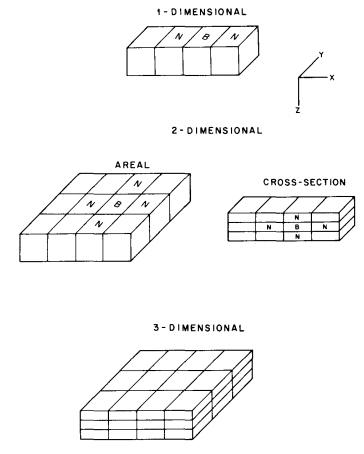
\includegraphics[width=.6\textwidth]{figs/revisao/revisao_DIM}
	\caption{Classifica\c{c}\~{a}o dos simuladores por dimens\~{a}o \cite{coats1982} \label{fig:revisao_DIM}}
\end{figure}

\'{E} importante que, ao se escolher um simulador num\'{e}rico para se resolver problemas de engenharia de reservat\'{o}rio, se considere v\'{a}rios fatores, a saber: o tipo de estudo a ser feito, tipo e caracter\'{i}sticas do reservat\'{o}rio e dos fluidos presentes, quantidade e qualidade dos dados, o detalhamento necess\'{a}rio do estudo e os recursos computacionais dispon\'{i}veis \cite[p. 519]{engres}. Por exemplo, \'{e} impratic\'{a}vel o uso de modelos composicionais em computadores cuja capacidade seja compar\'{a}vel a um computador pessoal de alto desempenho, devido \`{a} complexidade dos c\'{a}lculos envolvidos. Por outro lado, por sua simplicidade, um modelo \textit{black oil} poderia ser considerado, respeitando-se ao m\'{a}ximo as caracter\'{i}sticas do reservat\'{o}rio estudado.

\subsection{Uso de Simuladores Num\'{e}ricos para Estudos de Reservat\'{o}rios}

O uso de simuladores num\'{e}ricos torna poss\'{i}vel analisar o comportamento de um reservat\'{o}rio ao longo do tempo, dado um esquema de produ\c{c}\~{a}o. Dessa forma, pode-se obter, por exemplo, as condi\c{c}\~{o}es \'{o}timas de produ\c{c}\~{a}o, al\'{e}m de se determinar como a inje\c{c}\~{a}o de diferentes tipos de fluidos ou outros m\'{e}todos de EOR afetam o sistema simulado, determinar o efeito da localiza\c{c}\~{a}o dos po\c{c}os na recupera\c{c}\~{a}o de \'{o}leo e/ou g\'{a}s e analisar a influ\^{e}ncia de diferentes vaz\~{o}es de produ\c{c}\~{a}o e/ou inje\c{c}\~{a}o. O simulador obt\'{e}m seus resultados de informa\c{c}\~{o}es de natureza geol\'{o}gica, propriedades da rocha e dos fluidos presentes no meio poroso, hist\'{o}ricos de produ\c{c}\~{a}o (vaz\~{o}es e/ou produ\c{c}\~{o}es acumuladas de \'{o}leo e \'{a}gua) e de press\~{a}o, e outras informa\c{c}\~{o}es a respeito dos po\c{c}os de petr\'{o}leo, assim como as caracter\'{i}sticas de completa\c{c}\~{a}o \cite[pp. 522--523]{engres}. A Figura \ref{fig:revisao_simsec1} ilustra a aplica\c{c}\~{a}o de simuladores num\'{e}ricos para engenharia de reservat\'{o}rios.

\begin{figure}[!ht]
	\centering
	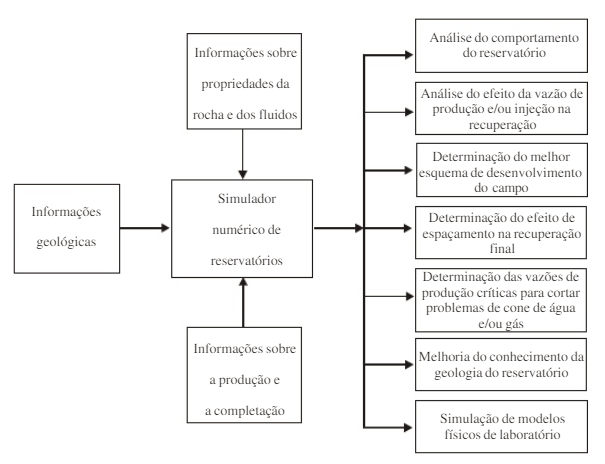
\includegraphics[width=.75\textwidth]{figs/revisao/revisao_simsec1}
	\caption{Aplica\c{c}\~{a}o de simuladores num\'{e}ricos em reservat\'{o}rios \cite[p. 522]{engres}}
	\label{fig:revisao_simsec1}
\end{figure}  

As etapas normalmente seguidas durante a simula\c{c}\~{a}o num\'{e}rica de um reservat\'{o}rio s\~{a}o \footnote{Ver \cite[pp. 523--524]{engres}.}:

\begin{enumerate}
\item \textbf{Coleta e prepara\c{c}\~{a}o dos dados:} \'{e} a fase de armazenamento e interpreta\c{c}\~{a}o de todos os dados cab\'{i}veis ao problema, sejam eles geol\'{o}gicos, propriedades da rocha e dos fluidos, entre outros. Quanto maiores a quantidade e a qualidade desses dados, mais confi\'{a}vel ser\'{a} a simula\c{c}\~{a}o. Breitenbach destaca que dados adicionais podem ser necessários considerando-se a dificuldade do problema de mecânica dos fluidos e os objetivos de estudo, dependentes de qual processo do reservatório está sendo modelado \cite{breitenbach1991}.
\item \textbf{Prepara\c{c}\~{a}o do modelo num\'{e}rico:} Ocorre logo ap\'{o}s a tomada dos dados. Inicialmente, \'{e} feito o \textit{lan\c{c}amento do} grid \textit{ou malha}, onde \'{e} constru\'{i}da uma malha para se transpor as informa\c{c}\~{o}es necess\'{a}rias para o modelo. Logo, \'{e} feita a divis\~{a}o do reservat\'{o}rio em v\'{a}rias c\'{e}lulas, cada uma funcionando como um reservat\'{o}rio menor, conforme mostra a Figura \ref{fig:revisao_simsec3}.
\begin{figure}[H]
	\centering
	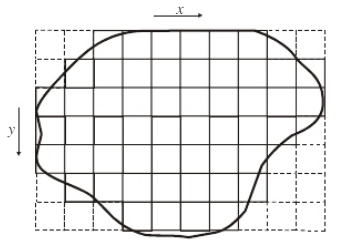
\includegraphics[width=.5\textwidth]{figs/revisao/revisao_simsec3}
	\caption{Malha utilizada na simula\c{c}\~{a}o num\'{e}rica de um reservat\'{o}rio \cite[p. 524]{engres}}
	\label{fig:revisao_simsec3}
\end{figure}
\item \textbf{Ajuste de hist\'{o}rico:} O objetivo desta etapa \'{e} calibrar o modelo num\'{e}rico com o reservat\'{o}rio real a partir dos melhores dados dispon\'{i}veis referentes aos hist\'{o}ricos de produ\c{c}\~{a}o e de press\~{a}o. O ajuste de hist\'{o}rico \'{e} um c\'{a}lculo do comportamento passado do reservat\'{o}rio e a consequente compara\c{c}\~{a}o com o hist\'{o}rico do campo ou do mesmo reservat\'{o}rio. Se a concord\^{a}ncia n\~{a}o \'{e} satisfat\'{o}ria, s\~{a}o necess\'{a}rios ajustes nos dados at\'{e} se obter resultados adequados. De todo modo, a import\^{a}ncia de se obter um bom ajuste de hist\'{o}rico reside no fato de que o modelo poder\'{a} ser utilizado para se efetuar previs\~{o}es confi\'{a}veis em rela\c{c}\~{a}o ao seu comportamento futuro.
\item \textbf{Extrapola\c{c}\~{a}o:} Uma vez que o ajuste de hist\'{o}rico \'{e} realizado, procede-se \`{a} fase de extrapola\c{c}\~{a}o, isto \'{e}, a previs\~{a}o de comportamento futuro do modelo. Podem ser impostas vaz\~{o}es e press\~{o}es para todos os po\c{c}os, condi\c{c}\~{o}es dessas vaz\~{o}es, entre outros. Essa etapa permite avaliar v\'{a}rios esquemas de produ\c{c}\~{a}o, e seus resultados podem ser utilizados em avalia\c{c}\~{o}es econ\^{o}micas, tornando poss\'{i}vel decidir pelo esquema \'{o}timo de produ\c{c}\~{a}o.
\end{enumerate}

Todas as etapas de simula\c{c}\~{a}o num\'{e}rica de reservat\'{o}rios est\~{a}o resumidos na Figura \ref{fig:revisao_simsec2}.

\begin{figure}[!ht]
	\centering
	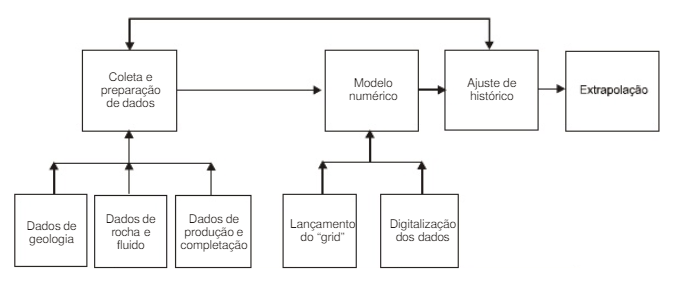
\includegraphics[width=.75\textwidth]{figs/revisao/revisao_simsec2}
	\caption{Etapas da simula\c{c}\~{a}o num\'{e}rica de um reservat\'{o}rio \cite[p. 523]{engres}}
	\label{fig:revisao_simsec2}
\end{figure}